\documentclass[english,11pt,usenames,dvipsnames]{beamer}

\DeclareMathOperator{\Cov}{Cov}
\DeclareMathOperator{\Var}{Var}
\DeclareMathOperator{\E}{\mathbb{E}}
\DeclareMathOperator{\Proba}{\mathbb{P}}

\newcommand{\Covb}[2]{\ensuremath{\Cov\!\left[#1,#2\right]}}
\newcommand{\Eb}[1]{\ensuremath{\E\!\left[#1\right]}}
\newcommand{\Pb}[1]{\ensuremath{\Proba\!\left[#1\right]}}
\newcommand{\Varb}[1]{\ensuremath{\Var\!\left[#1\right]}}

% norm
\newcommand{\norm}[1]{\| #1 \|}

\newcommand{\indep}{\rotatebox[origin=c]{90}{$\models$}}





\usepackage{mathptmx,amsmath,amssymb,graphicx,bibentry,bbm,babel,ragged2e}

\makeatletter

\newcommand{\noun}[1]{\textsc{#1}}
\newcommand{\jitem}[1]{\item \begin{justify} #1 \end{justify} \vfill{}}
\newcommand{\sframe}[2]{\frame{\frametitle{#1} #2}}

\newenvironment{centercolumns}{\begin{columns}[c]}{\end{columns}}
%\newenvironment{jitem}{\begin{justify}\begin{itemize}}{\end{itemize}\end{justify}}

\usetheme{Warsaw}
\setbeamertemplate{footline}[text line]{}
\setbeamercolor{structure}{fg=purple!50!blue, bg=purple!50!blue}

\setbeamersize{text margin left=15pt,text margin right=15pt}

\setbeamercovered{transparent}

\setbeamertemplate{headline}{}
\setbeamertemplate{footline}[frame number]
\setbeamertemplate{navigation symbols}{}

\@ifundefined{showcaptionsetup}{}{%
 \PassOptionsToPackage{caption=false}{subfig}}
\usepackage{subfig}

\usepackage[utf8]{inputenc}
\usepackage[T1]{fontenc}


\usepackage{tikz}

\usepackage{multirow}


\usepackage{mdframed}

\usepackage[usenames,dvipsnames]{pstricks}
\usepackage{auto-pst-pdf}


\usepackage[dvipsnames]{xcolor}


\makeatother

\begin{document}


\title{De l'endogénéité des hiérarchies dans les systèmes territoriaux complexes}

\author{J.~Raimbault$^{1,2,3}$\\
\texttt{juste.raimbault@iscpif.fr}
}


\institute{$^{1}$UPS CNRS 3611 ISC-PIF\\
$^{2}$CASA, UCL\\
$^{3}$UMR CNRS 8504 G{\'e}ographie-cit{\'e}s
}


\date{Journée de l'Institut de Géographie\\\smallskip
3 avril 2019
}

\frame{\maketitle}

%\textbf{Mots-clés : }\textit{Théories de la complexité ; théorie évolutive urbaine ; lois d'échelle}



%Le concept de hiérarchie émerge naturellement au sein de différentes théories et modèles des systèmes complexes.

\sframe{Hiérarchies territoriales}{

% intro simple - coole le nouveau geoportail - et puis je suis fascine par les cartes - topo on voit deja une structure socio-eco des territoires ; du systeme de villes. en chanegant d'echelle, une imbruication de systemes se revele : des variations de taille suggerent deja l'idee d'une hierrchie urbaine.

% opening slide : basic example - system of cities ?
% -> classic map example

\centering

\includegraphics[width=0.44\textwidth]{figures/intro_paname.png}\hspace{0.05cm}
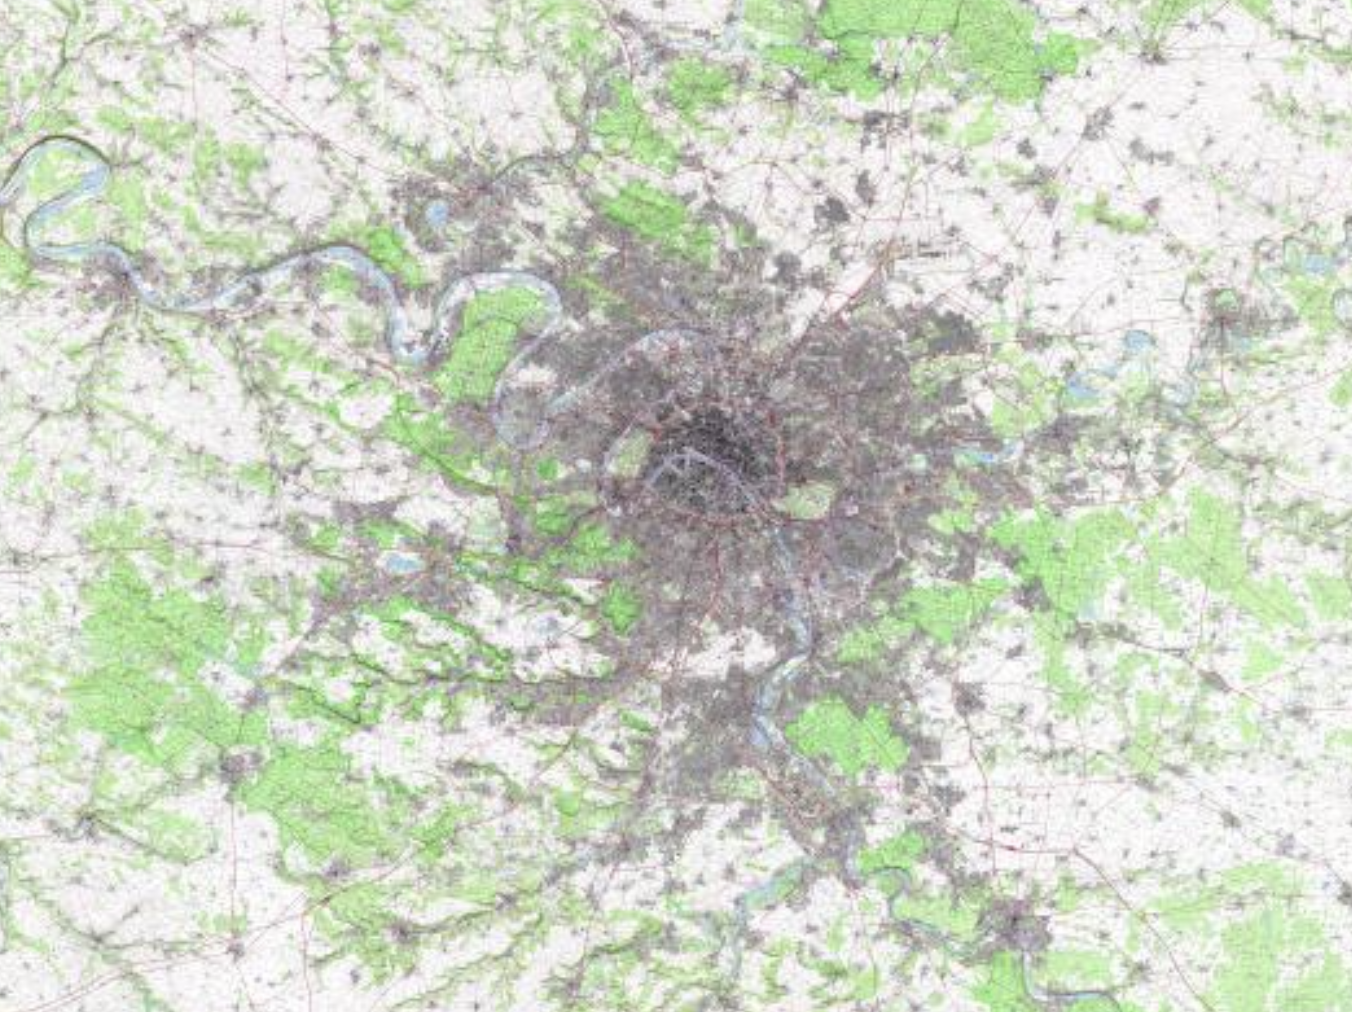
\includegraphics[width=0.45\textwidth]{figures/intro_bp.png}\\
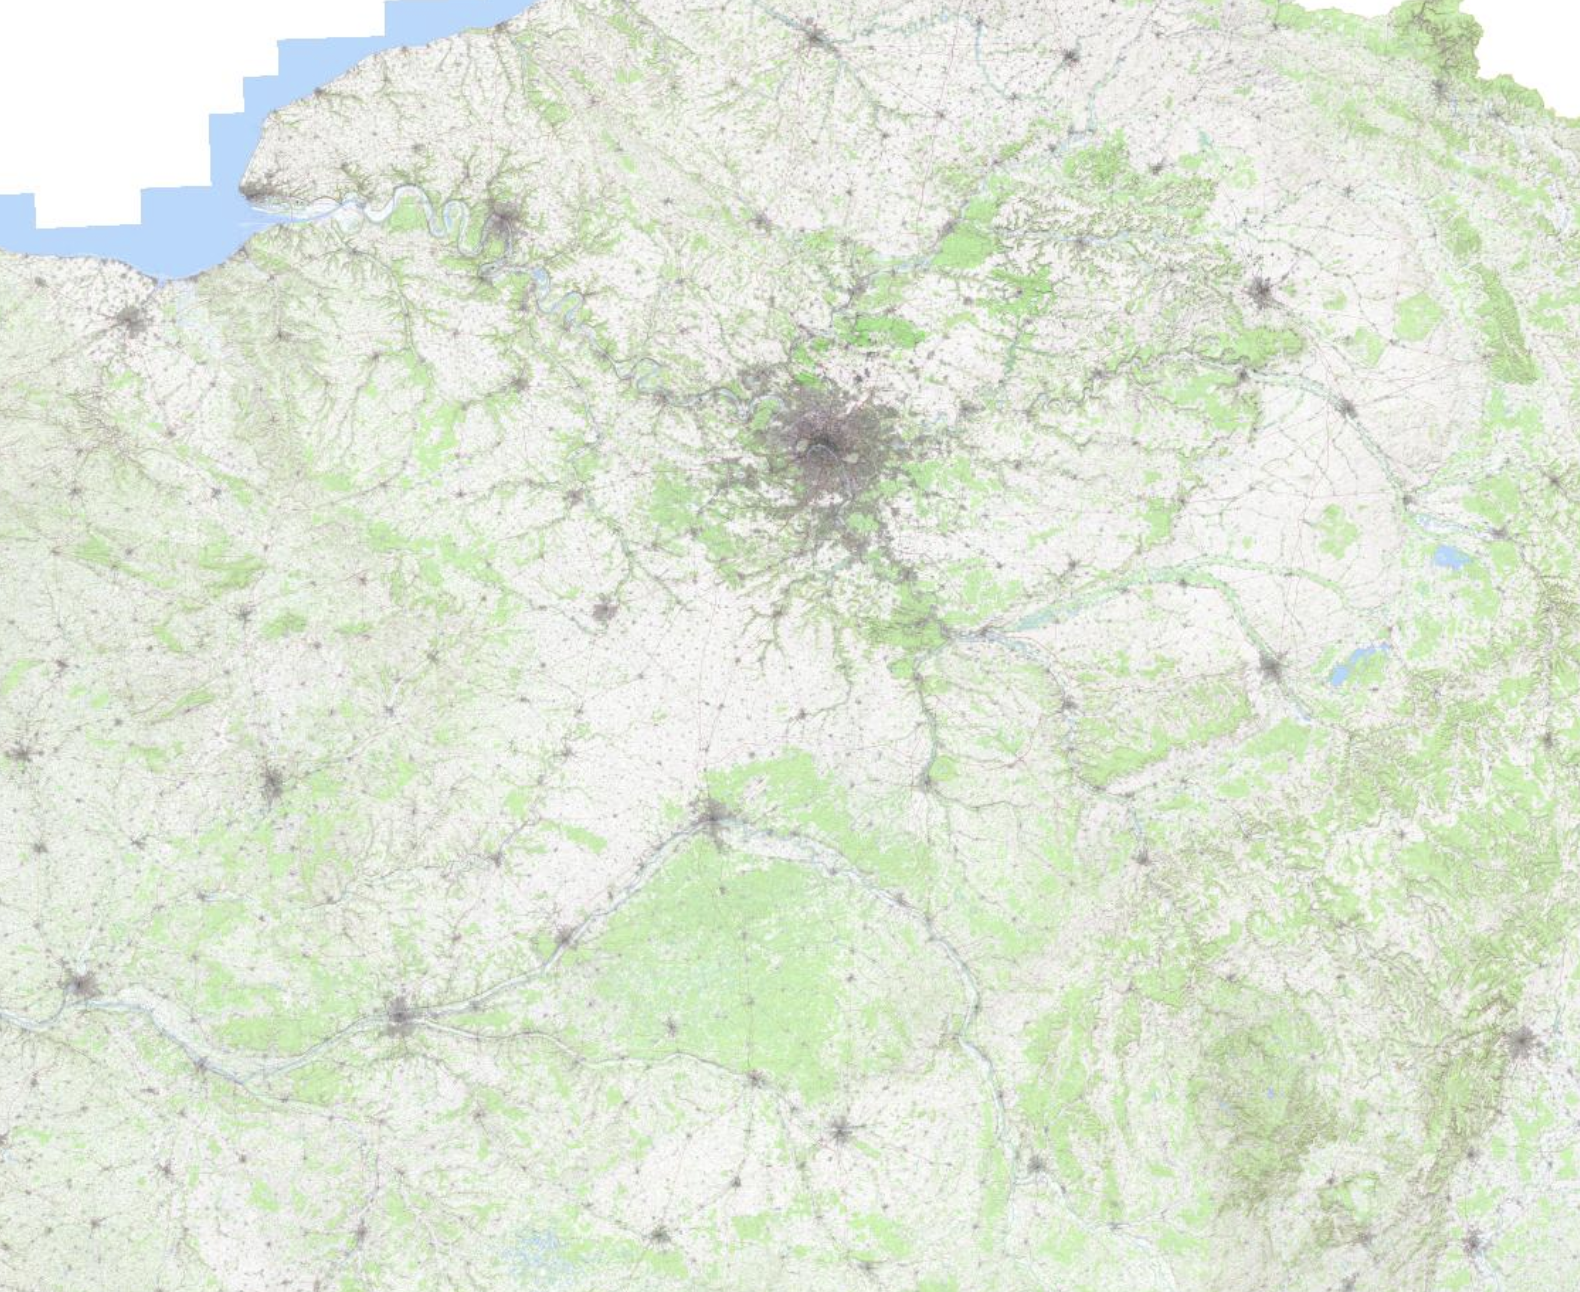
\includegraphics[width=0.45\textwidth]{figures/intro_northfr.png}\hspace{0.05cm}
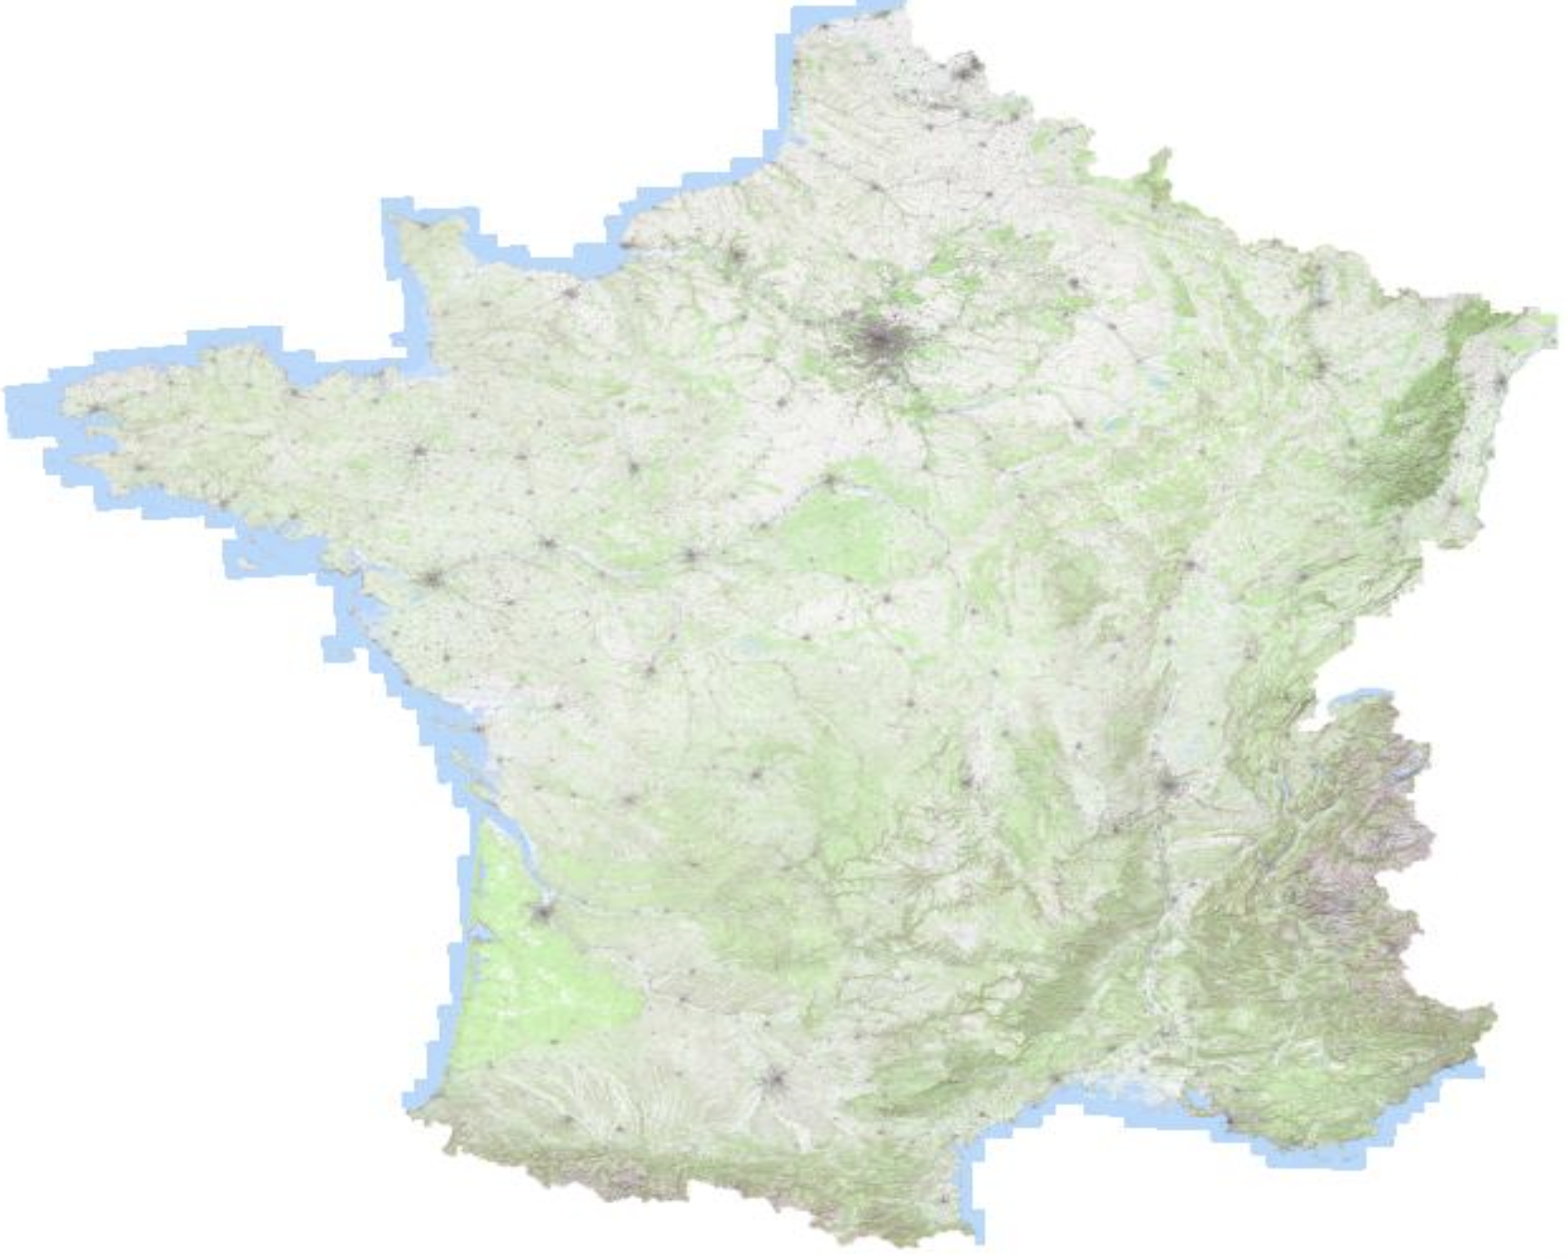
\includegraphics[width=0.45\textwidth]{figures/intro_fr.png}

\tiny \textit{Source: Geoportail}


}


\sframe{Définition(s) de la hiérarchie}{

% il m'incombe la lourde tache d'ouvrir la journee et donc de proposer au moins une premiere definition - vision - approche de la hierarchie. Il ne semble pas exister de definition claire ni unifiee - l'aac l'associe a des processus de categoristaion, qui impliquent necessairement des hierarchies entre categories.
% domination : relation d'ordre ? dependance ?
% "hierarchie de l'info " : processus de selection des donnees ; precategorisation : correspond a th multiscalaire de l'info ? si filtre info pas pertinente a cette echelle ?

% -> ce quil manque dans ce que je presente  reflexivite sur les outils de la demarche sci elle meme (en ouverture ? : systemes ou modeles des systemes ?)
% en fait si : la hierarchisation faite par le chercheur est endogene !


% different theories :
% - imbrication of systems and boundaries chez Holland
% - scaling, Zipf law en economie, geo.
% - theorie evolutive : diffusion hierarchique de l'innovation ?

% Def Hypergeo
% La notion de hiérarchie est employée avec deux sens distincts.
%C’est une organisation sociale, politique ou administrative en niveaux où chaque élément appartenant à un niveau est strictement subordonné à un élément du niveau supérieur. Plus l’on s’élève dans l’ordre du pouvoir ou de la domination et moins chaque niveau comporte d’éléments : la hiérarchie implique une organisation pyramidale. Cette forme d’organisation a l’avantage de permettre de faire circuler des informations ou d’imposer des décisions en réduisant les délais de transmission, elle a l’inconvénient d’une certaine rigidité dans l’adaptation au changement. En ce sens, les organisations hiérarchisées du travail dans les entreprises ou dans le fonctionnement de groupes sont parfois opposées aux organisations "en réseaux" (en dépit du fait qu’une hiérarchie soit une forme particulière de réseau), où les connexions sont plus nombreuses et qui ont plus de souplesse d’adaptation. Dans ce sens précis, les territoires présentent rarement une organisation hiérarchisée, excepté pour ce qui relève de l’organisation emboîtée de certains maillages administratifs. Par extension on appelle hiérarchie un système organisé selon une relation arborescente (c’est-à-dire qui se représente par un arbre au sens de la théorie des graphes), qui définit des sous-systèmes emboîtés, mais pas nécessairement subordonnés (par exemple dans une classification ascendante hiérarchique).
% La hiérarchie décrit aussi une forme d’organisation d’un système en sous-systèmes tels que le nombre de sous-systèmes varie selon une progression géométrique inverse du nombre des éléments (taille) de chaque sous-sytème. Les modèles statistiques de ces hiérarchies sont les distributions de Pareto, ou la distribution lognormale (dite de Galton-Gibrat). C’est la forme d’organisation la plus fréquente dans la nature. La taille des entreprises dans un secteur d’activité, la superficie des exploitations agricoles dans une région, la dimension des territoires dans le monde, la taille des villes dans un Etat...en sont des exemples en géographie. La hiérarchie urbaine, décrite par la loi rang-taille, ou la lieux est une forme particulièrement stable et universelle de l’organisation du peuplement et des activités dans un territoire.


% interesting : "social science hierarchy definition" in scholar : rapidly paper related to complex systems.

% phsicist def : 10.1371/journal.pone.0033799


% link hierarchy - complexity ?

%\cite{crumley1987dialectical}

\justify

\textit{Des définitions et concepts propres à chaque approche ?} Sciences politiques \cite{crumley1987dialectical}, Physique \cite{10.1371/journal.pone.0033799}, Systèmes complexes \cite{pumain2006hierarchy}, Science des villes \cite{batty2006hierarchy}



% - dialectical approach to hierarchy : metaphor, such as structure.
% - hierarchy in network : generalized centrality
% - Pumain 2006 ed : comeplx systems - natural/social
% - Batty

\bigskip
\bigskip

\textbf{Def. Hypergeo} : (i) organisation en structure arborescente, liens de subordination; (ii) organisation d'un système en sous-systèmes (\textit{émergence}), avec présence de lois d'échelle pour les propriétés des sous-systèmes.

\medskip

$\sim$ \textit{top-down simple / bottom-up complexe}

\bigskip
\bigskip

$\rightarrow$ \textit{des approches complémentaires mises en valeur au cours de la journée, quel niveau d'intégration possible ?}



}



\sframe{Des hiérarchies endogènes ?}{

%Cette contribution vise à illustrer dans quelle mesure une prise en compte de la complexité sociale ne peut en être dissociée. 

% Nous développons dans un premier temps des approches théoriques de la complexité.
% Dans un second temps, nous donnons des illustrations sur un plan thématique par des théories de l'organisation spatiale des systèmes territoriaux.
% => inverser pour la presentation (pedagogie)


% À la lumière de ces exemples, nous postulons que les hiérarchies, que ce soit au sens de l'imbrication de multiples niveaux ou échelles, ou de distributions statistiques à grande queue, sont endogènes aux systèmes territoriaux complexes.

$\rightarrow$ \textit{concept de hiérarchie étroitement lié à la complexité, l'émergence, les échelles multiples}

\bigskip


\textbf{La hiérarchie [le concept de] est-elle endogène aux systèmes (territoriaux) complexes ?}

\bigskip

\textit{Approche théorique :}

$\rightarrow$ exemples de théories complexes des villes

$\rightarrow$ généralisation à des théories des systèmes complexes



}


%La théorie évolutive des villes \citep{pumain2018evolutionary} nécessite d'une part l'intégration des multiples échelles des systèmes urbains (micro, meso, macro) pour expliquer les faits stylisés typiques connus sur les systèmes de villes, et d'autre part montre par l'application de modèles de simulation l'émergence de la hiérarchie à l'origine \citep{pumain2017simpoplocal} mais aussi lors de changements de régime comme l'apparition de nouveaux modes de transport \citep{raimbault2018modeling}.

\sframe{Théorie évolutive des villes}{

{\footnotesize Systèmes de villes comme systèmes complexes adaptatifs multi-échelles; principaux faits stylisés connus \cite{pumain2018evolutionary} et généricité \cite{pumain2015multilevel}
}

\medskip

\centering

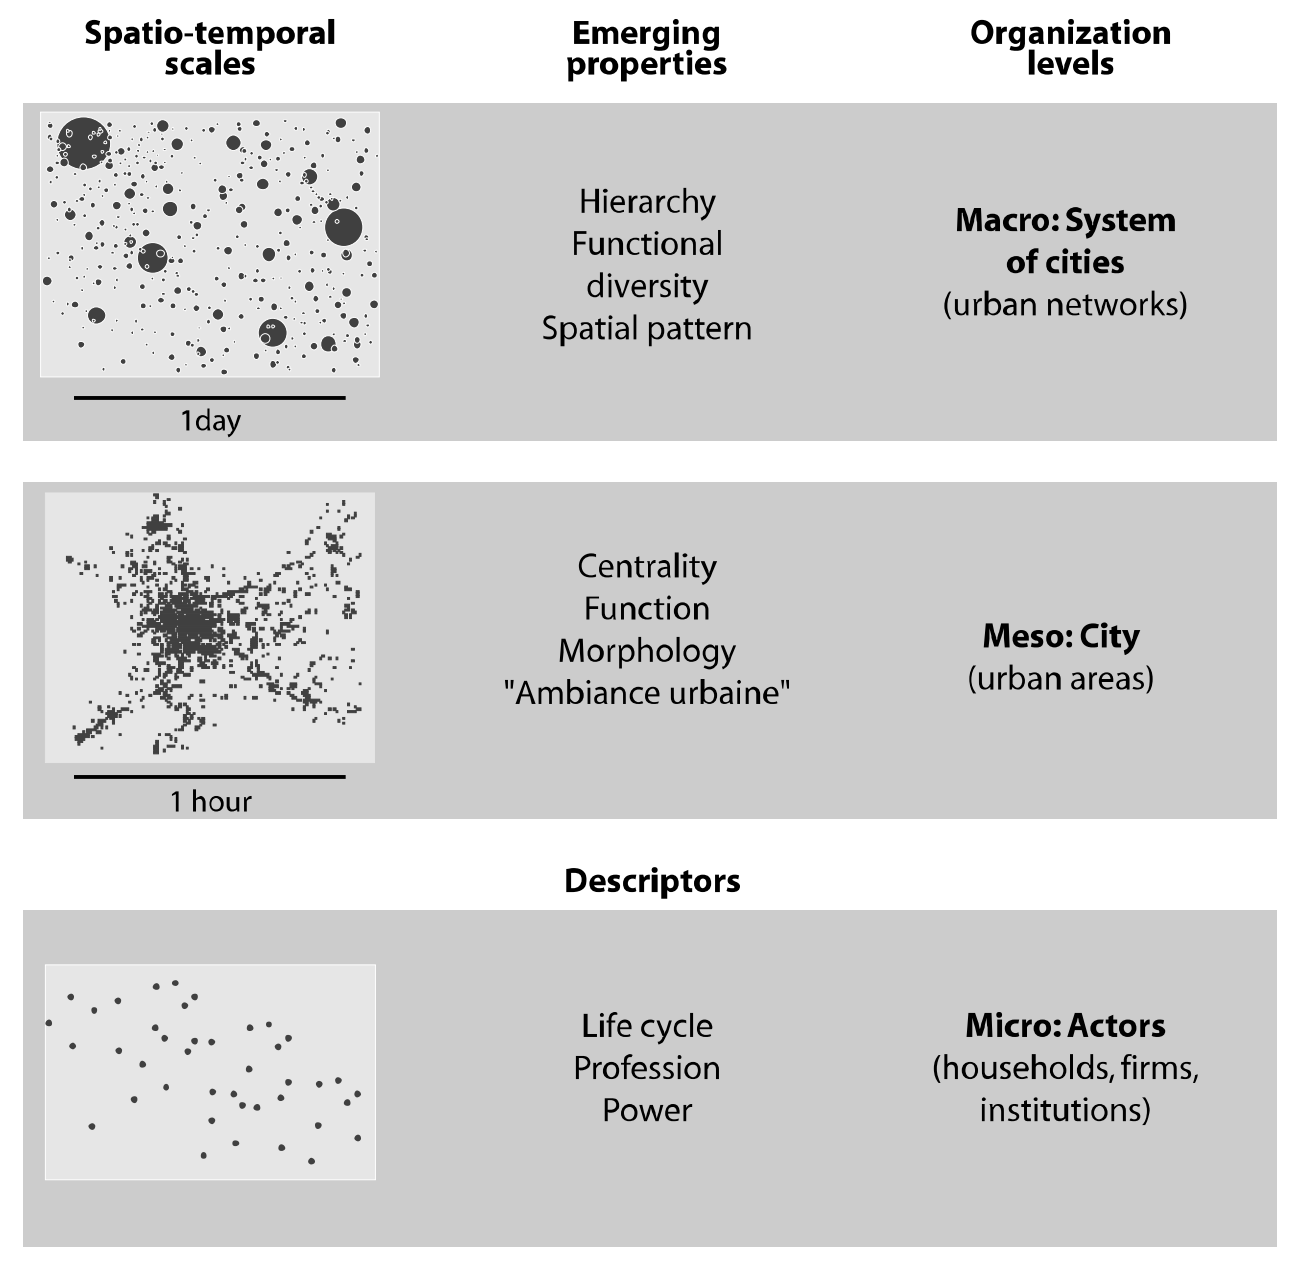
\includegraphics[width=0.5\textwidth]{figures/thevol_scales.png}\hspace{0.1cm}
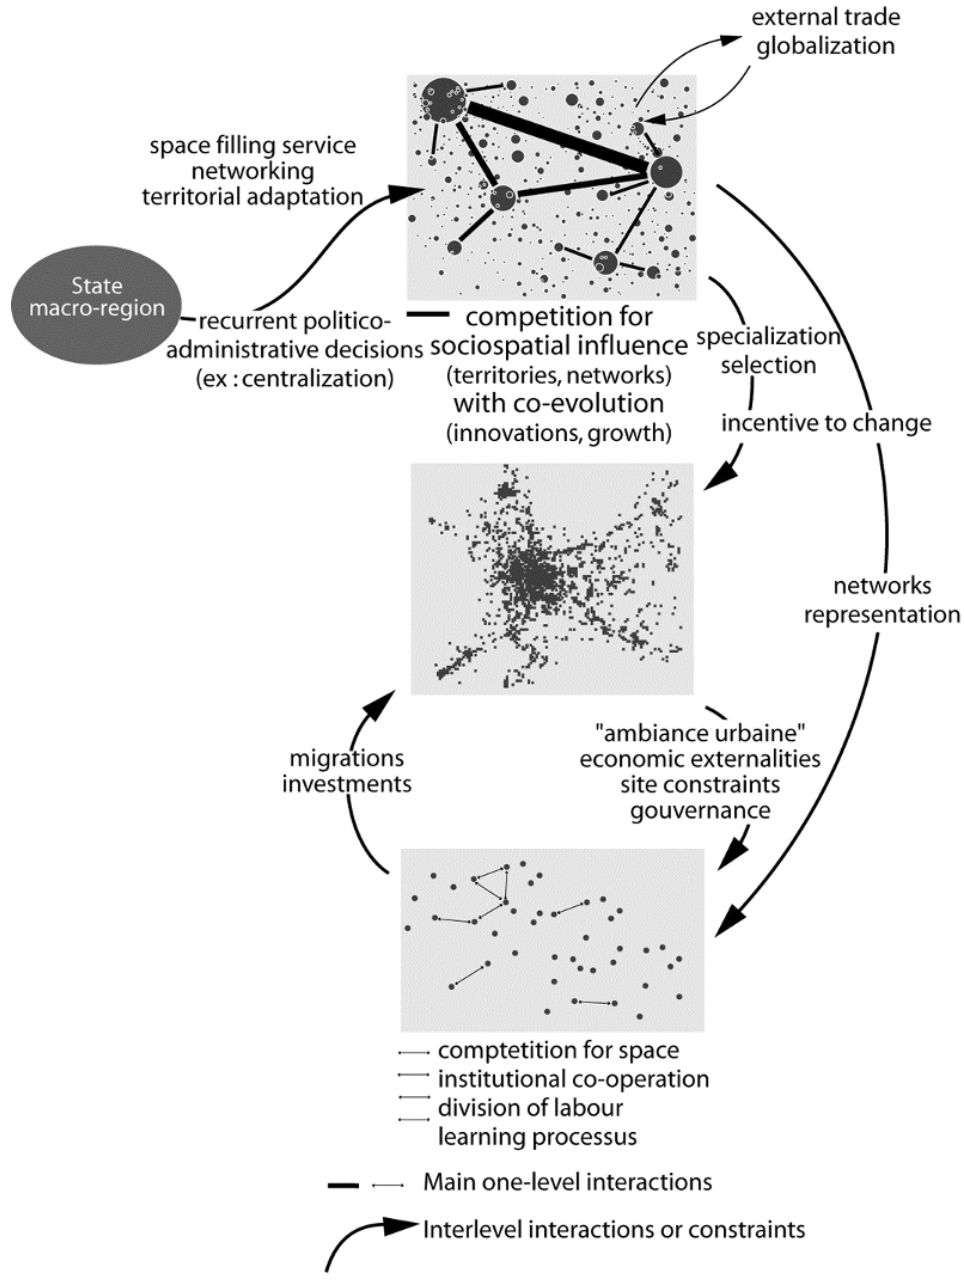
\includegraphics[width=0.4\textwidth]{figures/thevol_multiscale.png}


{\tiny
Source: \cite{pumain2008socio}
}

}

\sframe{Emergence de la hiérarchie}{

Modèle SimpopLocal pour l'émergence des systèmes de villes et de la hiérarchie \cite{pumain2017simpoplocal}

\medskip

\centering

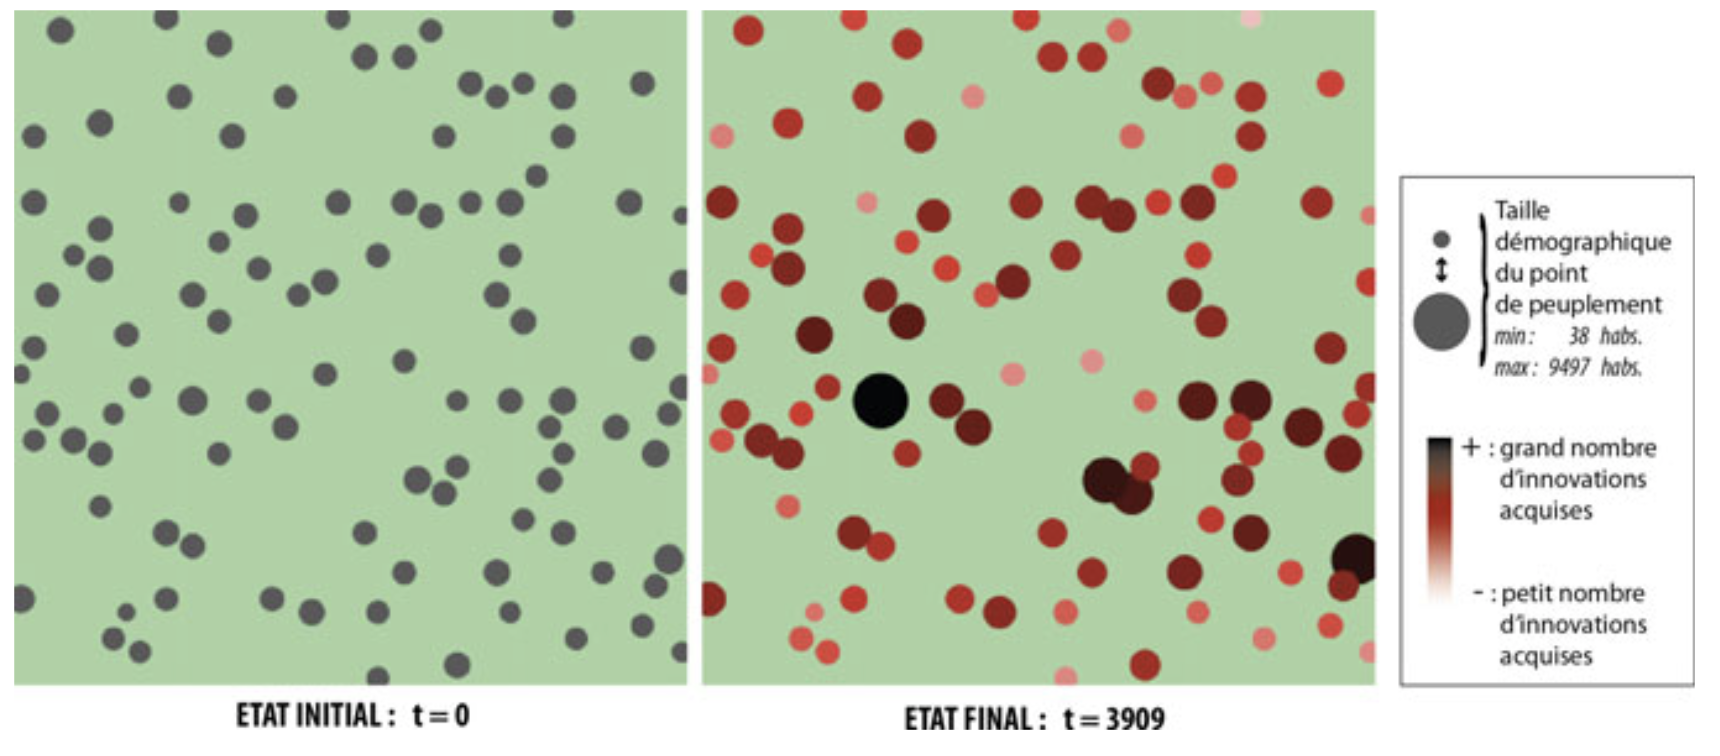
\includegraphics[width=\textwidth]{figures/thevol_simpoplocal.png}

{\tiny
Source: \cite{schmitt2014modelisation}
}

}





\sframe{Interaction réseaux-territoires}{

Renforcements ou inversions de hiérarchie liés à la co-évolution réseaux de transport-villes  \cite{raimbault2018indirect} \cite{raimbault2018modeling}


\centering

\bigskip
\bigskip

\begin{columns}
	\begin{column}{0.2\columnwidth}
		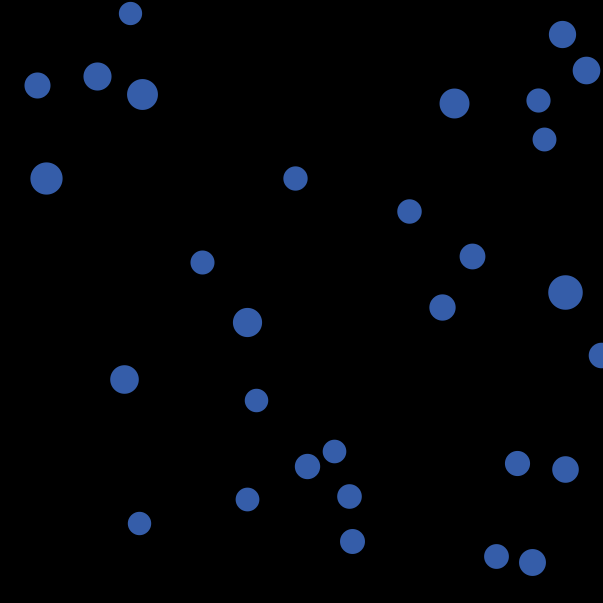
\includegraphics[width=\columnwidth]{figures/macrocoevol_example_virtual_0_t0.png}\\\vspace{0.05cm}
		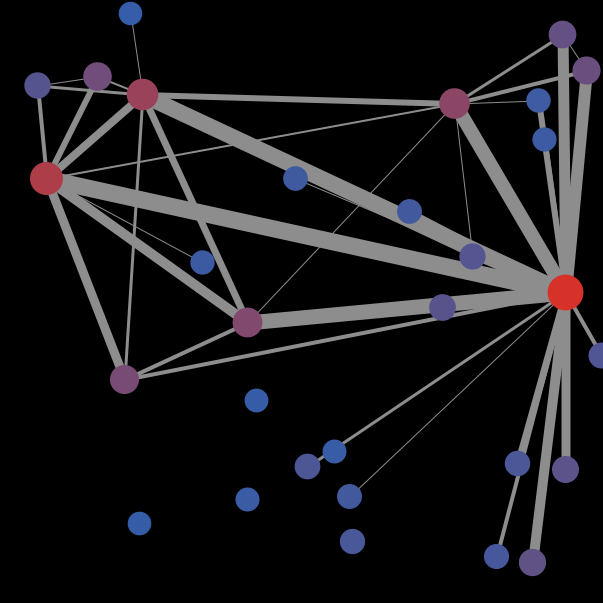
\includegraphics[width=\columnwidth]{figures/macrocoevol_example_virtual_0_tf.png}
	\end{column}
	%\hspace{0.2cm}
	\begin{column}{0.8\columnwidth}
		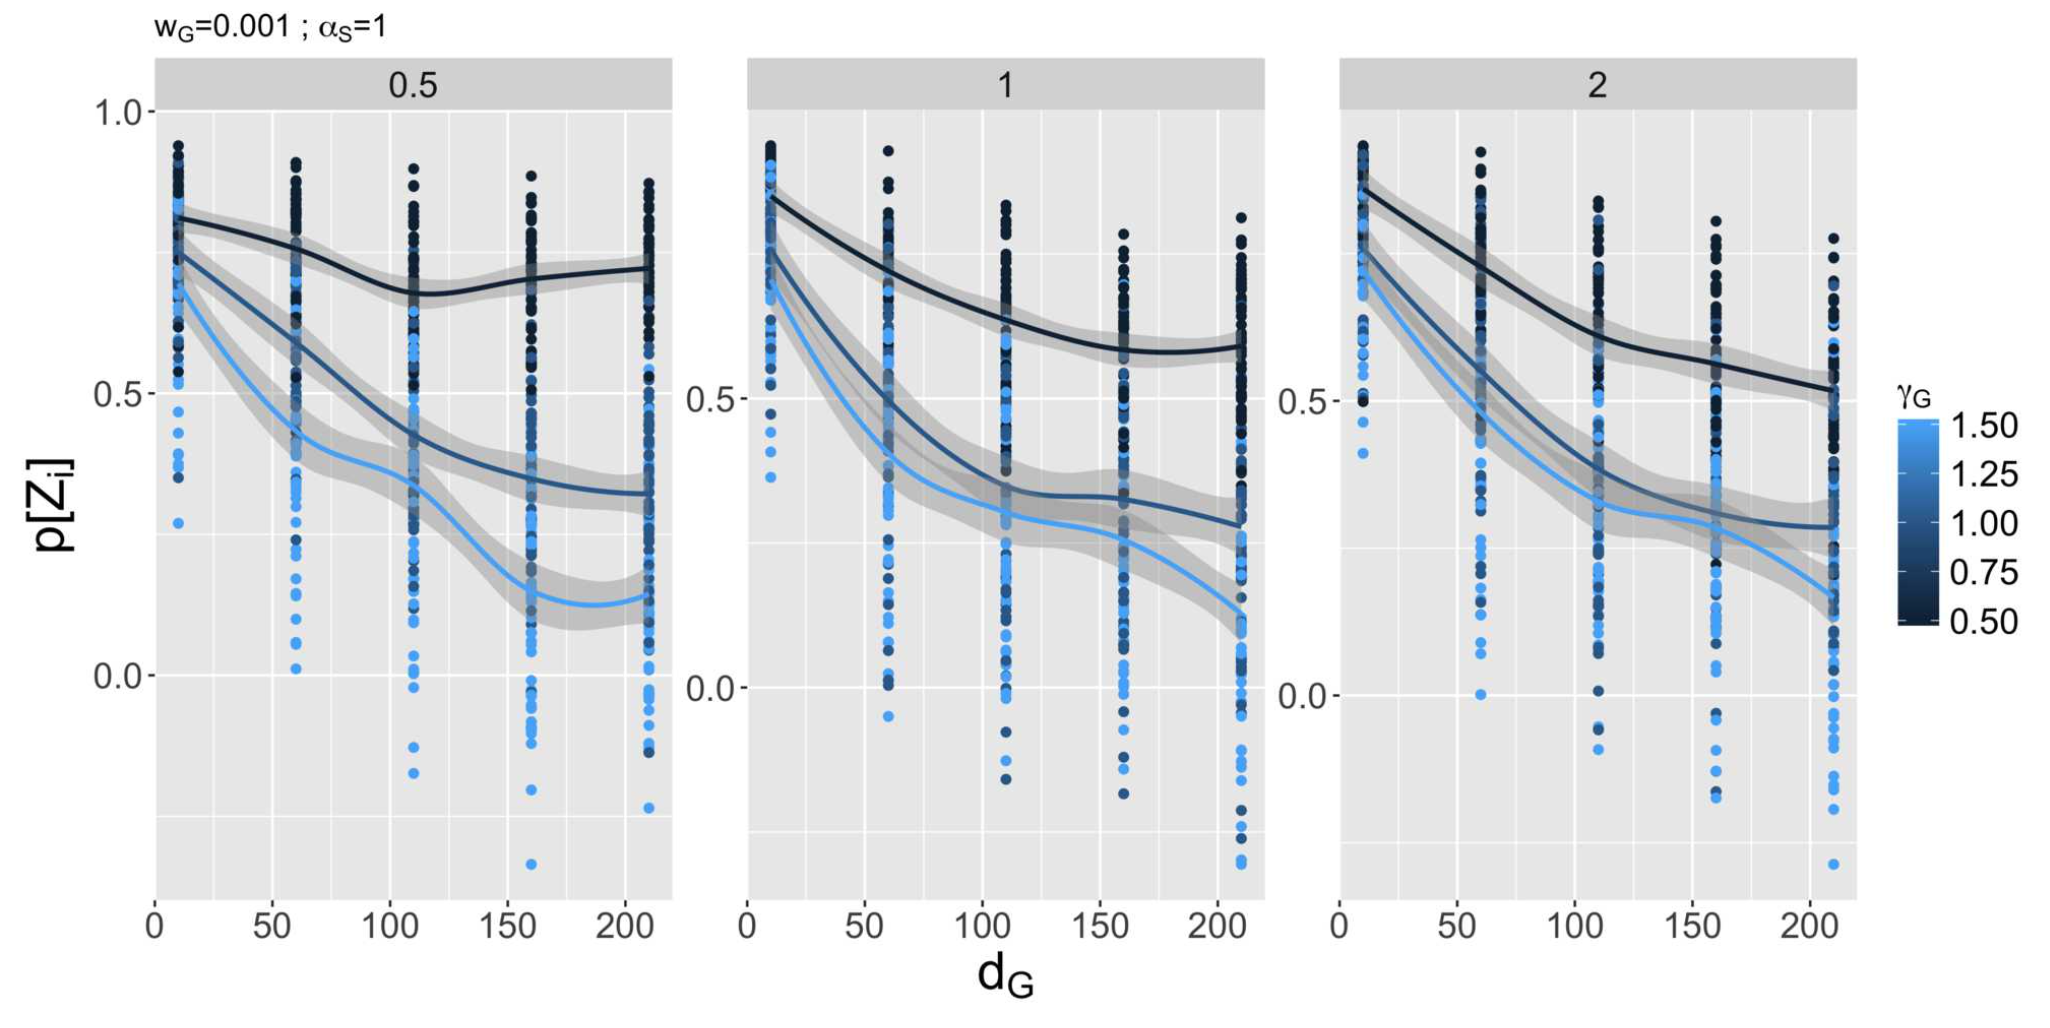
\includegraphics[width=\columnwidth]{figures/thevol_hierarchyinversion.png}
	\end{column}
\end{columns}

{\tiny
Source: \cite{raimbault2018modeling}
}

}




%La théorie des lois d'échelle, appliquée aux systèmes urbains par \cite{bettencourt2007growth}, montre l'endogénéité des hiérarchies pour les activités bénéficiant du rôle d'incubateur social des villes.

\sframe{Théorie du Scaling}{

\justify

Lois d'échelle pour les systèmes urbains \cite{bettencourt2007growth} : scaling infra et supra linéaire émerge selon les types d'activités, selon la définition des villes \cite{cottineau2017diverse}

\centering

\bigskip
\bigskip

\begin{columns}
	\begin{column}{0.5\textwidth}
		\centering
		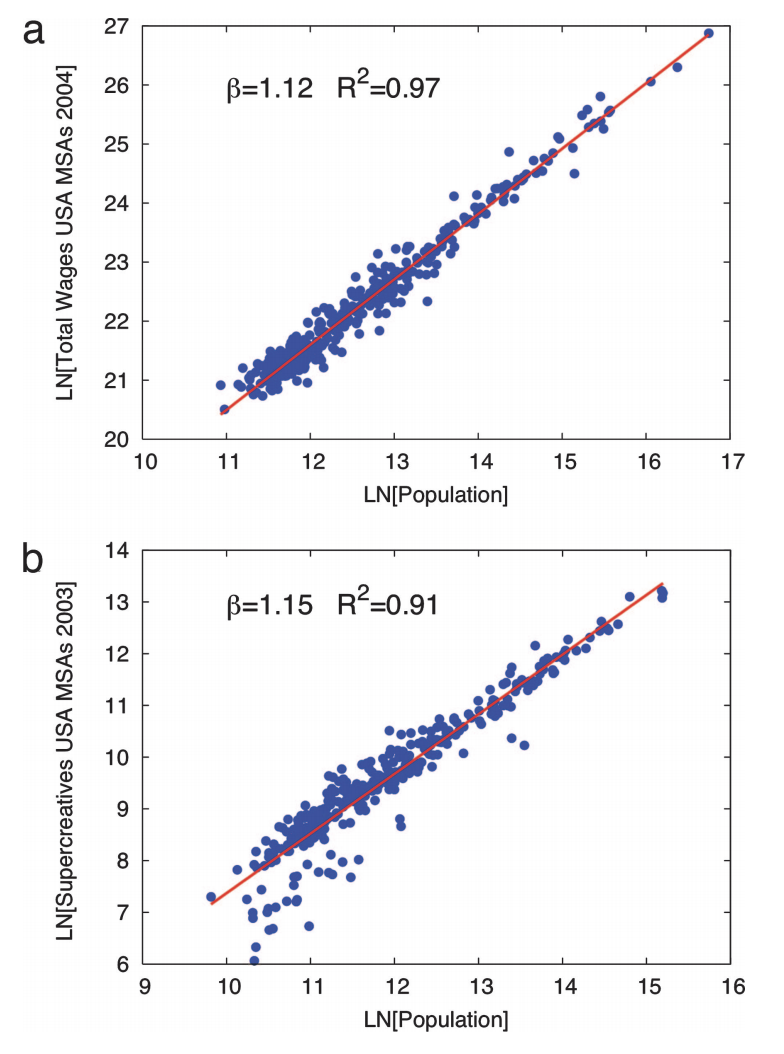
\includegraphics[width=0.5\linewidth]{figures/scaling_west0.png}
		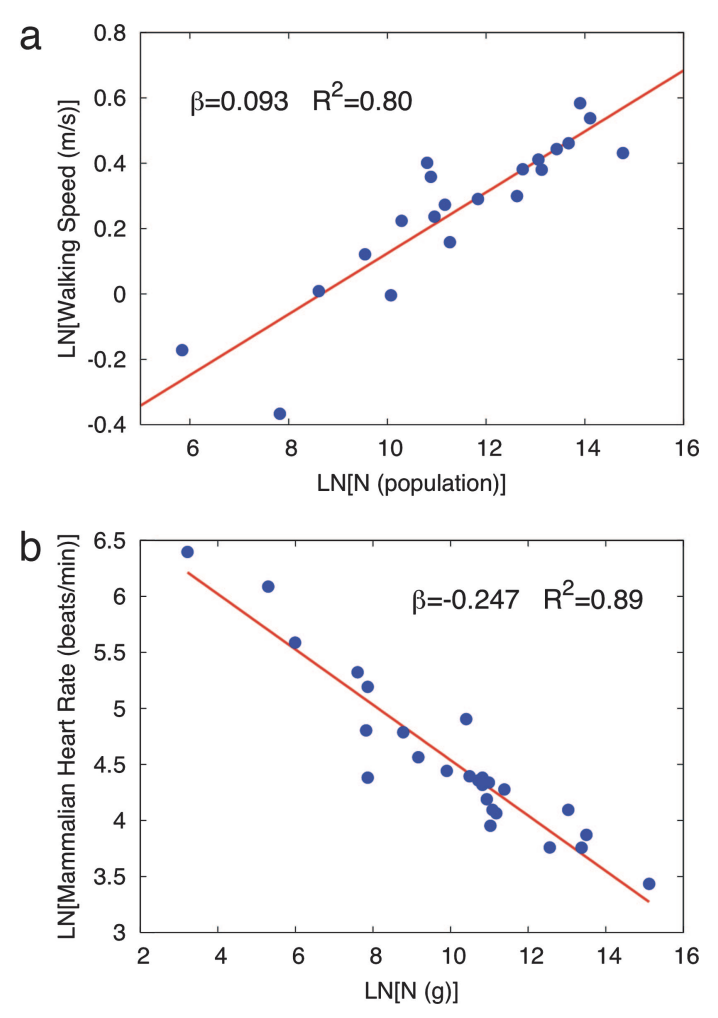
\includegraphics[width=0.5\linewidth]{figures/scaling_west1.png}
		
		{\tiny \cite{bettencourt2007growth}}
	\end{column}
	\begin{column}{0.5\textwidth}
		\centering
		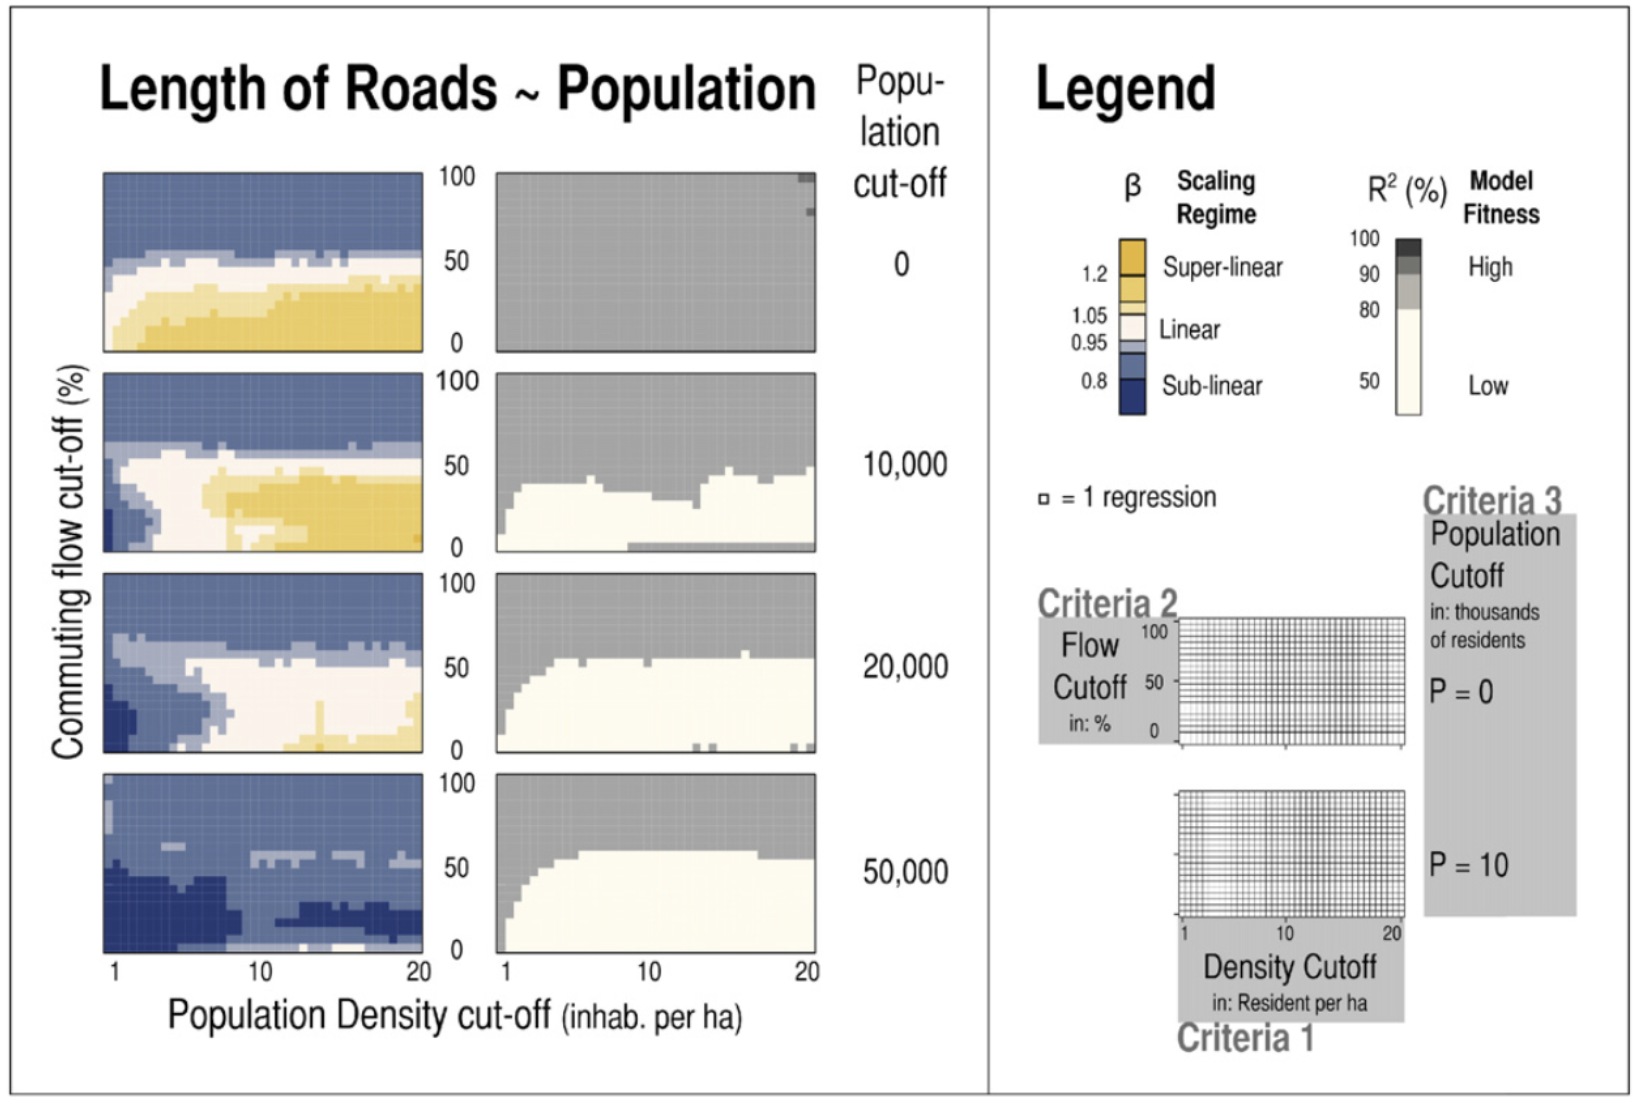
\includegraphics[width=\linewidth]{figures/scaling_cottineau.png}
		
		{\tiny \cite{cottineau2017diverse}}
	\end{column}
\end{columns}


%{\tiny
%Source: Left \cite{bettencourt2007growth}, Right \cite{cottineau2017diverse}
%}

}

% À la lumière de ces exemples, nous postulons que les hiérarchies, que ce soit au sens de l'imbrication de multiples niveaux ou échelles, ou de distributions statistiques à grande queue, sont endogènes aux systèmes territoriaux complexes.





%%%%%%
%% Generalization


%La théorie des systèmes complexes adaptatifs de \cite{holland2012signals}, considère l'imbrication des niches, dont les frontières filtrent les signaux entre celles-ci, comme des briques élémentaires de systèmes multi-niveaux par essence hiérarchiques. Cette approche s'applique par exemple autant aux systèmes écologiques qu'aux systèmes territoriaux.

\sframe{Systèmes complexes adaptatifs}{

% -> schema ?

\justify

Théorie des systèmes complexes adaptatifs de \cite{holland2012signals} : imbrication de sous-systèmes s'échangeant des signaux, filtrés par les frontières; sous-systèmes comme niches de co-évolution.


\centering

\smallskip

\includegraphics[width=0.8\textwidth]{figures/cas}

% TODO signaux aussi entre les niveaux ? pas de raison que non

{\tiny
d'après \cite{holland2012signals}
}

}



%La théorie multiscalaire de l'information introduite par \cite{allen2017multiscale} utilise la distribution de l'information entre les différents niveaux du système comme une méthode pour caractériser son niveau de complexité, et montre que les profils complexes sont justement ceux présentant une articulation entre les différentes échelles et une hiérarchie.

\sframe{Théorie multiscalaire de l'information}{

Théorie multiscalaire de l'information \cite{allen2017multiscale} : distribution et partage de l'information entre les composants d'un système caractérise sa complexité

\centering

\medskip

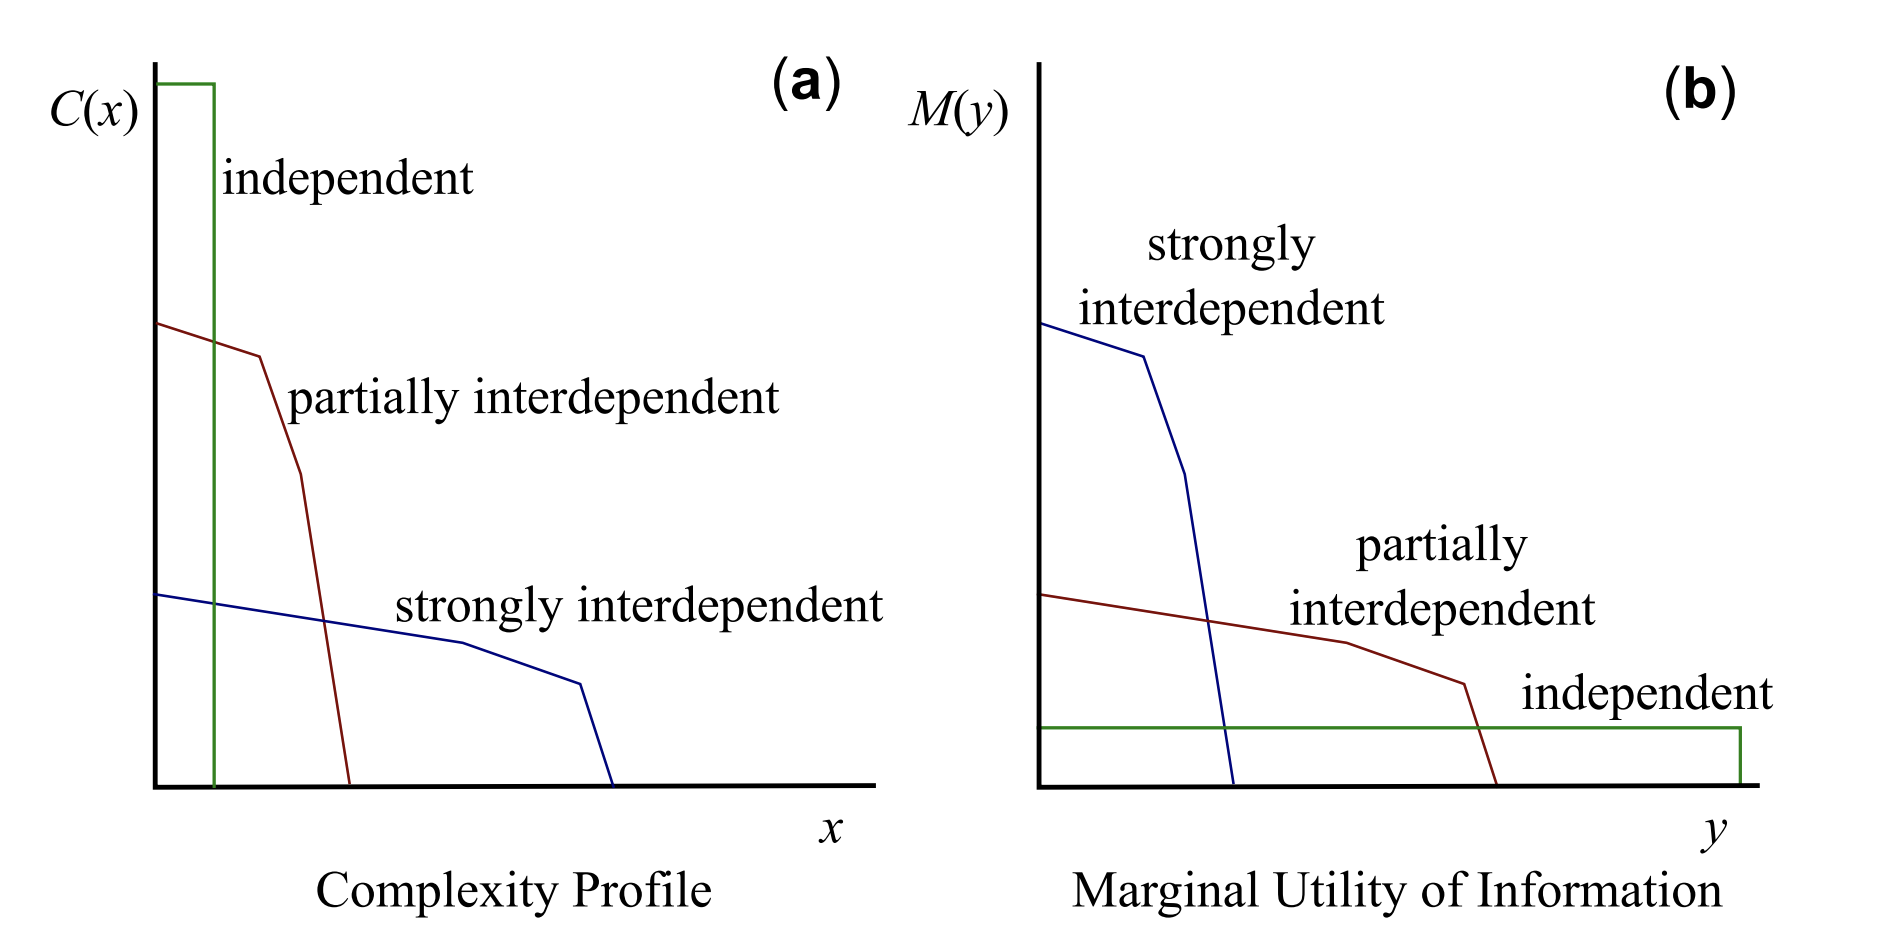
\includegraphics[width=0.9\textwidth]{figures/multiscaleinfo.png}

{\tiny
\textit{Profil de complexité: quantité d'information selon l'échelle.} Source: \cite{allen2017multiscale}
}

}



%D'autres approches moins formalisées insistent également sur le rôle de la hiérarchie, comme \cite{morin1980methode} qui montre la tension entre dépendance et indépendance d'un organisme à ses constituants, à l'ensemble des niveaux.


\sframe{Complexité Morinienne}{

Dans La Méthode \cite{morin1980methode} :

\bigskip

\begin{itemize}
	\item construction complexe et hiérarchique d'une méthode de la connaissance interdisciplinaire
	\item tension entre dépendance et indépendance pour l'ensemble des systèmes complexes
	\item ouverture / fermeture (rejoint \cite{holland2012signals})
	\item hiérarchie des systèmes sociaux: vers des sociétés du troisième type?
\end{itemize}


}





% À la lumière de ces exemples, nous postulons que les hiérarchies, que ce soit au sens de l'imbrication de multiples niveaux ou échelles, ou de distributions statistiques à grande queue, sont endogènes aux systèmes territoriaux complexes.

%Il fait alors difficilement sens de proposer que le concept de hiérarchie serait entièrement exogène. En termes d'aide à la décision, et notamment en termes de structures sociales ou politiques, la remise en question complete de la hiérarchie associée aux propositions d'organisations purement horizontales, n'est ni basée sur des faits ni compatible avec les théories de la complexité, en opposition avec les besoins actuels de modèles multi-scalaires pour l'intelligence territoriale soutenable \citep{rozenblat2018conclusion}.

%Ainsi, des approches plus intégratives, larges dans la portée des systèmes considérés, et basées sur les faits, ne peuvent complètement déconstruire le concept de hiérarchie de par son endogénéité à la complexité.


\sframe{Discussion}{

\justify

\textbf{Proposition : } \textit{les hiérarchies, au sens d'imbrication de sous-systèmes à de multiples niveaux, sont endogènes aux systèmes complexes}

\bigskip

$\rightarrow$ des structures ``hiérarchiques'' au sens commun (structure de dépendance rigide et arborescente) sont simples et ni adaptatives ni résilientes

\smallskip

$\rightarrow$ le concept de hiérarchie ne peut être considéré comme exogène et totalement déconstruit

\smallskip

$\rightarrow$ pour l'aide à la décision, des utopies réductionnistes en horizontalité complète s'opposent aux théories de la complexité

\smallskip

$\rightarrow$ question ouverte (reflexive): endogènes \textit{aux systèmes} ou aux \textit{théories et modèles des systèmes} ?


\bigskip

\textbf{Des approches multi-scalaires intégratives pour des gouvernances territoriales soutenables \cite{rozenblat2018conclusion} doivent prendre en compte la complexités des hiérarchies.}
% et la complexite de la hieraachie ? rq : ce pattern revient souvent en sci sociales ?

% rq : en se placant dans ces cadres de la complexite, tout ce qui est dit ici sont des banalités ? - du coup ce serait endogene a l'approche prise ? pas que, puisque empiriquement on montre que la hierarchie a émergé. mais on le montre car on a le bon concept. tourne en rond - application du knowledge framework.

}





% pas besoin de slide cl -> discussion
%\sframe{Conclusion}{

%\bigskip

%\footnotesize
%\textbf{Références}


%Raimbault, J. (2018). Calibration of a density-based model of urban morphogenesis. PloS one, 13(9):e0203516

%\bigskip
%\footnotesize{ - Code, données et résultats disponibles à\\ \texttt{https://github.com/JusteRaimbault/SpatialComplexity}\\
% - Article à \texttt{https://github.com/JusteRaimbault/SpatialComplexity/Docs/}\\\texttt{Rochebrune2019/Versions/Rochebrune2019{\_}Raimbault{\_}v1.pdf}\\
%- Remerciements à \textit{European Grid Infrastructure} et ses \textit{National Grid Initiatives} (\textit{France-Grilles} en particulier) pour le support technique et l'infrastructure.
%}
%}








%%%%%%%%%%%%%%%%%%%%%
\begin{frame}[allowframebreaks]
\frametitle{References}
\bibliographystyle{apalike}
\bibliography{biblio}
\end{frame}
%%%%%%%%%%%%%%%%%%%%%%%%%%%%










\end{document}







